\begin{center}
\small
\begin{figure}
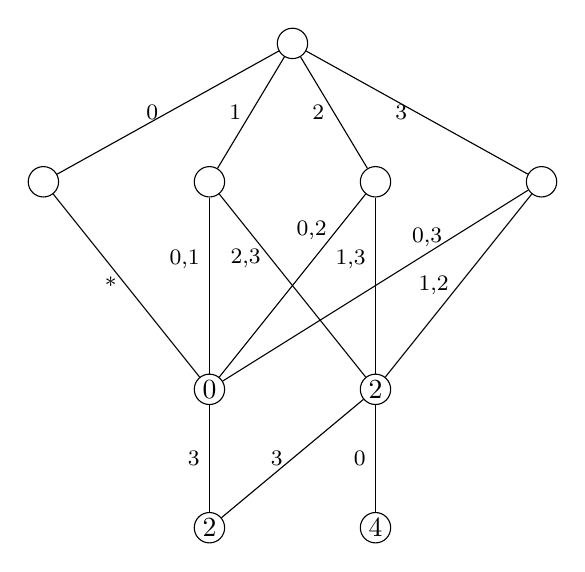
\begin{tikzpicture}[grow=down, level distance=50pt, edge from parent/.style={draw, -latex}]

    \node (S) [shape=circle,draw,inner sep=1pt] {\phantom{0}};
    \node at (-90pt, -50pt) (S0) [shape=circle,draw,inner sep=1pt] {\phantom{0}};
    \node at (-30pt, -50pt) (S1) [shape=circle,draw,inner sep=1pt] {\phantom{0}};
    \node at (30pt, -50pt) (S2) [shape=circle,draw,inner sep=1pt] {\phantom{0}};
    \node at (90pt, -50pt) (S3) [shape=circle,draw,inner sep=1pt] {\phantom{0}};
    \node at (-30pt, -125pt) (S00) [shape=circle,draw,inner sep=1pt] {0};
    \node at (30pt, -125pt) (S12) [shape=circle,draw,inner sep=1pt] {2};

    \node at (-30pt, -175pt) (F2) [shape=circle,draw,inner sep=1pt] {2};
    \node at (30pt, -175pt) (F4) [shape=circle,draw,inner sep=1pt] {4};

    \path[draw] (S) -- (S0) node [midway, left, font=\footnotesize] {0};
    \path[draw] (S) -- (S1) node [midway, left, font=\footnotesize] {1};
    \path[draw] (S) -- (S2) node [midway, left, font=\footnotesize] {2};
    \path[draw] (S) -- (S3) node [midway, left, font=\footnotesize] {3};
    \path[draw] (S0) -- (S00) node [midway, left, font=\footnotesize] {*};
    \path[draw] (S1) -- (S00) node [pos=0.35, left, font=\footnotesize] {0,1};
    \path[draw] (S1) -- (S12) node [pos=0.35, left, font=\footnotesize] {2,3};
    \path[draw] (S2) -- (S00) node [pos=0.2, left, font=\footnotesize] {0,2};
    \path[draw] (S2) -- (S12) node [pos=0.35, left, font=\footnotesize] {1,3};
    \path[draw] (S3) -- (S00) node [pos=0.25, left, font=\footnotesize] {0,3};
    \path[draw] (S3) -- (S12) node [midway, left, font=\footnotesize] {1,2};
    \path[draw] (S00) -- (F2) node [midway, left, font=\footnotesize] {3};
    \path[draw] (S12) -- (F2) node [midway, left, font=\footnotesize] {3};
    \path[draw] (S12) -- (F4) node [midway, left, font=\footnotesize] {0};

\end{tikzpicture}
\caption{Full quaternary tree.}
\end{figure}
\end{center}
